\chapter{Strata całkowita i uczenie}\label{rozdz:uczenie}

\section{Jak z pięciu głowic zrobić jedną liczbę?}

Sieć ma pięć głowic, każda ze swoją stratą (rozdział~\ref{rozdz:strata}). Uczyć możemy tylko jedną liczbą, więc je sumujemy z wagami; po drodze musimy zadbać o dwie rzeczy: o rzadkie etykiety (waga klasy dodatniej) i o \emph{brakujące} etykiety (maski dostępności, rozdział~\ref{rozdz:dane}).
Potem opisujemy, jak wyglądało uczenie: skąd brano dane, jak je zniekształcano (augmentacje), jakim harmonogramem i jak wybrano model końcowy.

Po tym rozdziale umiesz: (i)~zapisać pełną funkcję straty Gen~6, (ii)~uzasadnić, że etykieta niedostępna nie daje gradientu, (iii)~policzyć całkowitą stratę z zapisanych składowych, (iv)~odczytać z dziennika uczenia przebieg trzech sesji.

\section{Strata całkowita}

Niech $\mathrm{valid}_t\in\{0,1\}$ oznacza, że klatka $t$ nie jest dopełnieniem krótkiego wycinka, a $a_g\in\{0,1\}$ --- czy dla danego przykładu dostępna jest etykieta głowicy $g$. Maska głowicy to $m_g(t,s)=\mathrm{valid}_t\,a_g$. Dla głowic z mapami (początek, brzmi, koniec):
\begin{equation}
  \mathcal L_g=\frac{\sum_{t,s}m_g(t,s)\;\ell_{\alpha_g}\big(p_g(t,s),\,y_g(t,s)\big)}{\sum_{t,s}m_g(t,s)},\qquad g\in\{\mathrm{on},\mathrm{fr},\mathrm{off}\},
\end{equation}
z wagami klasy dodatniej $\alpha_\mathrm{on}=4$, $\alpha_\mathrm{fr}=1$, $\alpha_\mathrm{off}=2$ (def.~\ref{def:bce}). Strata głośności to błąd kwadratowy $\mathcal L_\mathrm{vel}=\sum\mu(\hat v-y_\mathrm{vel})^2\big/\max(1,\sum\mu)$ z maską $\mu$ równą $1$ tylko tam, gdzie znana jest głośność.
Strata tabulatury to średnia $-\ln p_i(t)[c_i(t)]$ po parach (klatka, struna) z etykietą znaną ($c_i(t)\ge0$) i $a_\mathrm{tab}=1$. Całość:
\begin{equation}
  \boxed{\ \mathcal L=1{,}0\,\mathcal L_\mathrm{on}+1{,}0\,\mathcal L_\mathrm{fr}+0{,}5\,\mathcal L_\mathrm{off}+0{,}5\,\mathcal L_\mathrm{vel}+0{,}5\,\mathcal L_\mathrm{tab}\ }
  \label{eq:strata}
\end{equation}

\begin{twierdzenie}[Niedostępna etykieta nie daje gradientu]\label{tw:maska}
Jeśli $a_g=0$ dla wszystkich przykładów w paczce, to $\mathcal L_g$ nie zależy od parametrów sieci, a jej gradient wynosi $0$.
\end{twierdzenie}
\begin{pomyslDowodu}
Licznik jest sumą wyrazów pomnożonych przez maskę równą zero; mianownik też, więc trzeba ustalić konwencję dzielenia przez zero --- w kodzie mianownik jest zastąpiony przez $\max(1,\cdot)$.
\end{pomyslDowodu}
\begin{proof}
Przy $a_g=0$ mamy $m_g\equiv0$, więc
\begin{align*}
\mathcal L_g &= \frac{\sum m_g\,\ell}{\max\big(1,\sum m_g\big)}=\frac{0}{\max(1,0)}=0 && \pow{(maska zerowa)}\\
\nabla_{\vect\theta}\mathcal L_g &= \frac{\sum_{t,s}m_g\,\nabla_{\vect\theta}\ell}{\max(1,\cdot)}=\vect0. && \pow{(każdy składnik ma czynnik $m_g=0$)}
\end{align*}
Strata jest więc stałym zerem i nie wpływa na $\nabla\mathcal L$. Stąd w Gen~6, w którym żadne źródło nie ma etykiet głośności, głowica głośności pozostała w stanie początkowym i nie jest używana. To kończy dowód.
\end{proof}

\begin{naliczbach}
Składowe zapisane w dzienniku uczenia dla epoki $5$ (wartości na zbiorze uczącym): $\mathcal L_\mathrm{on}=0{,}0239$, $\mathcal L_\mathrm{fr}=0{,}0336$, $\mathcal L_\mathrm{off}=0{,}0227$, $\mathcal L_\mathrm{vel}=0$, $\mathcal L_\mathrm{tab}=0{,}123$. Ze wzoru~\eqref{eq:strata}:
$\mathcal L=0{,}0239+0{,}0336+0{,}5\cdot0{,}0227+0{,}5\cdot0+0{,}5\cdot0{,}123=0{,}1304$. Największy wkład ma tabulatura ($0{,}0615$, czyli $47\%$) mimo wagi $0{,}5$, bo jej strata jest najwyższa: wybór struny to trudne zadanie.
\end{naliczbach}

\section{Jak dobierano dane i zniekształcano}

\textbf{Paczka.} W każdym kroku losuje się $16$ wycinków po $192$ klatki ($4{,}46$ s, razem $71$ s dźwięku). Źródło losuje się z prawdopodobieństwami $0{,}5$ (klasyka), $0{,}3$ (GuitarSet), $0{,}2$ (środowiska gitarowe), a nagranie w obrębie źródła proporcjonalnie do długości. Epoka to $1000$ kroków.

\begin{figure*}[ht]
\centering
\begin{tikzpicture}[>=Stealth,font=\small]
  \tikzset{b/.style={blok,text width=21mm,minimum height=13mm,align=center,font=\footnotesize}}
  \node[b] (zr) {źródła:\\klasyka $0{,}5$\\GuitarSet $0{,}3$\\środowiska $0{,}2$};
  \node[b,right=6mm of zr] (wy) {$16$ wycinków\\po $192$ klatki};
  \node[b,right=6mm of wy] (au) {augmentacje\\(tab.~\ref{tab:augmentacje})};
  \node[b,right=6mm of au,fill=blue!8!white] (si) {sieć Gen~6\\$249\,219$ param.};
  \node[b,right=6mm of si] (st) {$5$ strat\\$\times$ maski $a_g$};
  \node[b,right=6mm of st,fill=orange!10!white] (op) {$\mathcal L$, gradient,\\przycięcie $\le1$,\\AdamW};
  \draw[wektor] (zr)--(wy); \draw[wektor] (wy)--(au); \draw[wektor] (au)--(si); \draw[wektor] (si)--(st); \draw[wektor] (st)--(op);
  \draw[wektor] (op.south) -- ++(0,-6mm) -| node[pos=0.25,below,font=\footnotesize]{nowe wagi $\vect\theta$ ($\times1000$ w epoce)} (si.south);
\end{tikzpicture}
\caption{Jeden krok uczenia Gen~6. Z trzech źródeł (wagi losowania w ramce) losuje się $16$ wycinków po $4{,}46$ s, zniekształca je augmentacjami, przepuszcza przez sieć, liczy pięć strat z maskami dostępności etykiet, sumuje je do $\mathcal L$, przycina gradient do normy $1$ i aktualizuje wagi optymalizatorem AdamW; po $1000$ takich krokach kończy się epoka.}
\label{rys:krok-uczenia}
\end{figure*}

\textbf{Augmentacje} (każda losowana niezależnie) zmieniają cechy i etykiety w kontrolowany sposób, żeby sieć nie nauczyła się zapamiętywać:

\begin{table}[ht]
\centering\small
\begin{tabular}{@{}p{3.1cm}p{3.5cm}p{4.3cm}@{}}
\toprule
augmentacja & parametry & co symuluje\\
\midrule
poziom & $\pm6\dB$ ($+g/60$ do cech) & lokalnie cichszy/głośniejszy fragment\\
szum & $\sigma=0{,}02$ & szum cech\\
maska pasm i chwil & $15\%$ & utracone pasma i krótkie ubytki\\
tempo & $\times e^{u}$, $u\sim U(-\ln1{,}12,\ln1{,}12)$, $p=0{,}5$ & grę szybszą/wolniejszą\\
rozstrojenie & $\pm1$ bin ($\pm33$ centy), $p=0{,}3$ & gitarę rozstrojoną\\
niedokładne etykiety & początki/końce $\pm1$ klatka, $p=0{,}3$ & błędy adnotacji\\
transpozycja & $\pm2$ półtony, $p=0{,}3$ & inną tonację (tabulatura wtedy nieznana)\\
\bottomrule
\end{tabular}
\caption{Augmentacje użyte w uczeniu Gen~6 (konfiguracja \texttt{gen6\_kaggle.json}).}
\label{tab:augmentacje}
\end{table}

\begin{intuicja}
Augmentacja to „kłamstwo z kontrolowanym skutkiem”: wiemy, jak zmiana cech zmienia etykiety (albo że ich nie zmienia), więc możemy sztucznie mnożyć dane. Rozstrojenie przesuwa cechy o $1$ bin ($33$ centy), a etykiety zostają: sieć uczy się, że nuta rozstrojona o ćwierć półtonu to wciąż ta sama nuta.
\end{intuicja}

\begin{pulapka}
Augmentacja poziomu bywa mylona z niezależnością od głośności (tw.~\ref{tw:glosnosc}). Stałe przeskalowanie \emph{całego} nagrania jest już zneutralizowane przez normalizację. Augmentacja $\pm6\dB$ zmienia głośność \emph{wycinka względem referencji całego nagrania}, czyli symuluje, że ten fragment jest cichszy niż reszta utworu (dynamika), a nie że cały utwór jest cichszy.
\end{pulapka}

\section{Przebieg uczenia}

Uczenie przebiegło w trzech sesjach (pomijając przerwaną sesję~2), razem $97$ epok po $1000$ kroków (czasy z dziennika epok: $7{,}3+2{,}4+9{,}5\approx19$ godzin na GPU Tesla T4, mieszana precyzja fp16; dokumentacja projektu podaje $7{,}3+2{,}9+11\approx21$ godzin łącznie z uruchamianiem sesji).
\begin{itemize}
\item Sesja~1: epoki $0$--$35$ ($36$ epok), $\eta_0=10^{-3}\to0$ (kosinus, rozdział~\ref{rozdz:optymalizacja}); dane: zestaw~1 klasyki, środowiska, GuitarSet.
\item Sesja~3: epoki $36$--$47$ ($12$ epok), restart $\eta=4\cdot10^{-4}$, dodano drugi zestaw klasyki i augmentacje tempa, rozstrojenia i jittera etykiet; zatrzymana przez mechanizm wczesnego zatrzymania po $12$ epokach bez poprawy rekordu (to było niezamierzone: plan zakładał dłuższe uczenie).
\item Sesja~4: epoki $48$--$96$ ($49$ epok), $\eta=3\cdot10^{-4}\to0$ z harmonogramem liczonym od czasu.
\end{itemize}
Dobrym wynikiem uczenia jest to, co widać na rys.~\ref{rys:uczenie}: F1 nut na walidacji rośnie z $69{,}7\%$ (epoka~0) do $84{,}2\%$ (epoka~5), $88{,}3\%$ (epoka~20), $89{,}4\%$ (epoka~29, najlepsza w sesji~1); po restarcie w sesji~3 spada (dane trudniejsze, $\eta$ wyższy), a w sesji~4 znów rośnie do rekordu $90{,}27\%$ w epoce $81$.
Straty uczące maleją jak $\log_{10}$: tabulatura z $0{,}61$ do $0{,}046$, początki z $0{,}056$ do $0{,}021$.

\begin{figure*}[ht]
\centering
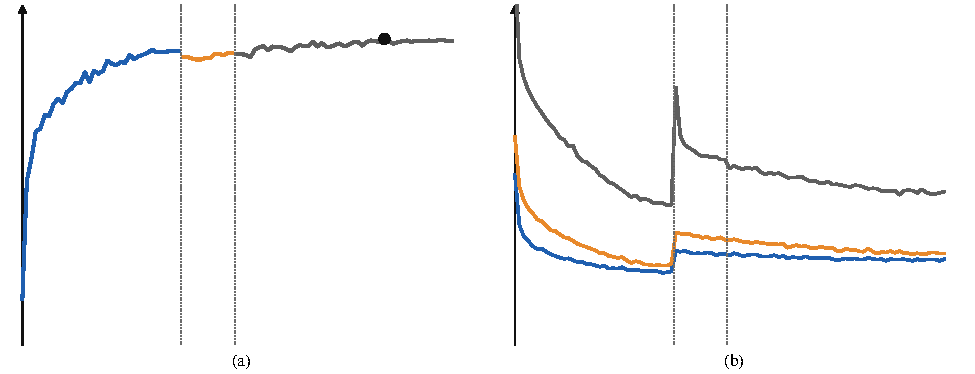
\includegraphics[width=\linewidth]{figures/uczenie.pdf}
\caption{Prawdziwy przebieg uczenia Gen~6 (dziennik \texttt{docs/wyniki/epoki.csv}, $97$ epok). (a) F1 nut na stałej próbie walidacyjnej $180$ nagrań (skala od $66$ do $93\%$): sesja~1 niebieska, sesja~3 pomarańczowa, sesja~4 ciemnoszara; czarna kropka to wybrana epoka $81$ ($90{,}27\%$). Pionowe linie rozdzielają sesje.
(b) $\log_{10}$ strat uczących: początki (niebieska), brzmi (pomarańczowa), tabulatura (ciemnoszara). Skok strat na początku sesji~3 i~4 to efekt restartu kroku i nowych, trudniejszych danych.}
\label{rys:uczenie}
\end{figure*}

\textbf{Wybór modelu.} Po każdej epoce liczono F1 nut na stałej próbie walidacyjnej ($180$ nagrań ze wszystkich źródeł) i zapamiętywano najlepszą epokę: $81$ ($90{,}27\%$). To jest model końcowy (plik \texttt{best.pt}, $249\,219$ parametrów).
Uczciwie: próba walidacyjna zawiera tylko $12$ nagrań prawdziwej gitary, więc istnieje niewielkie ryzyko dopasowania wyboru epoki do walidacji; wyniki końcowe liczymy osobno na zbiorze testowym (rozdział~\ref{rozdz:wyniki}).

\section*{Podsumowanie}
\begin{itemize}
\item $\mathcal L=1{,}0\mathcal L_\mathrm{on}+1{,}0\mathcal L_\mathrm{fr}+0{,}5\mathcal L_\mathrm{off}+0{,}5\mathcal L_\mathrm{vel}+0{,}5\mathcal L_\mathrm{tab}$, z maskami dostępności i ważoną BCE.
\item Niedostępna etykieta daje zerowy gradient (tw.~\ref{tw:maska}); głowica głośności pozostała nieuczona.
\item Paczka: $16\times192$ klatki, źródła $0{,}5/0{,}3/0{,}2$; augmentacje: poziom, szum, maski, tempo, rozstrojenie, jitter, transpozycja.
\item $97$ epok w trzech sesjach; najlepsza epoka $81$ ma F1 nut $90{,}27\%$ na walidacji.
\end{itemize}

\begin{sprawdz}
\begin{enumerate}
\item Dla epoki $20$: $\mathcal L_\mathrm{on}=0{,}0198$, $\mathcal L_\mathrm{fr}=0{,}0228$, $\mathcal L_\mathrm{off}=0{,}0193$, $\mathcal L_\mathrm{tab}=0{,}0545$, $\mathcal L_\mathrm{vel}=0$. Policz $\mathcal L$ i udział tabulatury.
\item Wycinek ma $192$ klatki, krok $256$ próbek przy $11\,025\Hz$. Ile sekund trwa? Ile sekund dźwięku jest w jednej paczce $16$ wycinków?
\item W paczce są $3$ nagrania z etykietami tabulatury i $13$ bez (maska $a_\mathrm{tab}=0$). Czy $\mathcal L_\mathrm{tab}$ uśrednia po wszystkich $16$ nagraniach? Uzasadnij.
\item Krok uczenia w sesji~4 wynosi $3\cdot10^{-4}\to0$ kosinusem od czasu. Ile wynosi w połowie czasu sesji?
\end{enumerate}
\end{sprawdz}

\subsection*{Rozwiązania}
\begin{enumerate}
\item $\mathcal L=0{,}0198+0{,}0228+0{,}0097+0+0{,}0273=0{,}0795$ (dokładnie $0{,}07950$); udział tabulatury $0{,}0273/0{,}0795=34\%$.
\item $192\cdot256/11\,025=4{,}46$ s; paczka: $16\cdot4{,}46=71{,}3$ s.
\item Nie: licznik i mianownik zawierają maskę, więc uśrednianie odbywa się tylko po parach (klatka, struna) z $a_\mathrm{tab}=1$, czyli po $3$ nagraniach; pozostałe $13$ nie wnoszą ani składnika, ani wagi (tw.~\ref{tw:maska}).
\item Połowa czasu: $q=0{,}5$, więc $\eta=3\cdot10^{-4}\cdot\tfrac12(1+\cos\tfrac\pi2)=1{,}5\cdot10^{-4}$.
\end{enumerate}
